\documentclass[UTF8]{ctexart}

\usepackage{subfiles}  

%下面的语句, 引入你的头部设置文件
\usepackage{C:/phpStorm_proj/02_myself_ID_EGO/+100_latex_all_math_sel/myPreamble} 
%必须是绝对路径, 才能让各个tex在单独编译时使用到

\title{物理}


%---------------------------------


\begin{document}
	\tableofcontents % 生成目录
	\date{} % 若不写这句, 则默认也会渲染出日期, 所以我们要手动赋空值
	\maketitle  %这行代码, 让你前面的 title, author, date生效
	
	
	\section{摆的等时性}
	
	摆的等时性 : 无论摆动的幅度大还是小, 完成一次摆动的时间是一样的.	
	
	各种机械摆钟, 就是根据这个原理制作的.
	
	摆绳越长, 往复摆动一次的时间(即周期), 也就越长.
	
	
~\\
\hrule
~\\
	
	
	
	\section{质量 mass}
	
	\textbf{质量: 物体所含物质的多少, 叫做``质量" mass.} 公式中就用其首字母 m 来表示. \\
	
	质量的单位是:	 \\
	- 1 t 吨 = 1000 kg \\
	- 1 kg 千克(即公斤) \\
	- 1 g 克 = 1000 mg \\
	- 1 mg 毫克 \\
	
	地球的质量 = $ 5.97237 \cdot 10^{24} \ kg $ \\
	太阳的质量 = $ 1.9891 \cdot 10^{30} \ kg $ \\
	
	称质量的工具: 秤  \\
	
	\textbf{质量无关``物态": 一块冰融化成水, 其质量不会改变.} \\	
	质量也无关``所处的位置": 一个东西在地球上, 或带到太空里, 其质量不会改变. \\
	即: 物体的质量, 不随它的物态, 位置而改变. 
	
	
	~\\
	\hrule
	~\\
	
	
	\section{$\text{密度}\rho =\frac{\text{质量}m}{\text{体积}V}$}
	
	同一种物体, 体积越大, 质量越大. \\
	密度 density : 由某种物质组成的物体的``质量", 与它``体积"之比, 就是这种物体的``密度". 
	
	\begin{align*}
		\boxed{
			\text{密度}\rho =\dfrac{\text{质量}m}{\text{体积}V}
		}
	\end{align*}

	这个公式就是说: \textbf{``密度"在数值上, 等于``物体单位体积的质量".} \\

	密度ρ的单位, 是由``质量的单位" 和 ``体积的单位" 共同组成的. 即, \textbf{密度的基本单位就是: $ kg/m^3$ (千克/立方米), 或 $ g/cm^3$ (克/立方厘米).} \\

	这两个密度单位的关系是: 
	\begin{align*}
		\boxed{			
		1 g / cm^3 = 1 \cdot 10^3 kg/m^3
		}
	\end{align*}
	1 克/立方厘米(克每立方厘米) = 1000 千克/立方米(千克每立方米) \\
	
	
	
	~\\
	\hrule
	~\\
	
	
	
	\section{大气压强}
	
	\subsection{标准大气压强 :  $1.013\cdot 10^5\ P_a$}
	
	大气压强, 简称为大气压(atmosphere), 或气压。\textbf{注意:大气压是"大气压强"的简称,不是"大气压力"的简称.} \\
	
	大气压产生的原因: 由于大气受到重力的作用而产生. \\
	大气压的方向: 同液体一样, 大气朝向各个方向都有压强的. \\
	
	
\includegraphics[width=0.3\textwidth]{img/0024.png}
	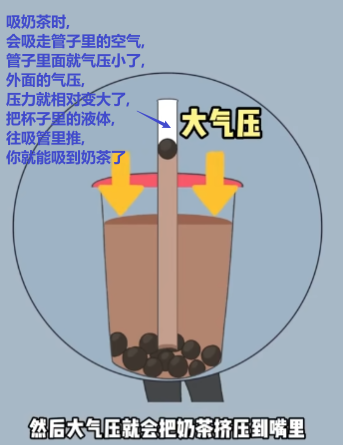
\includegraphics[width=0.3\textwidth]{img/0025.png}
	
	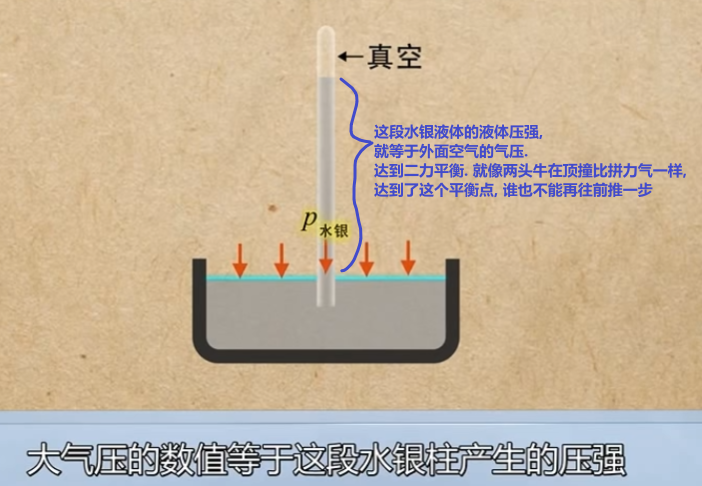
\includegraphics[width=0.3\textwidth]{img/0026.png}	
	
\includegraphics[width=0.3\textwidth]{img/0028.png}
	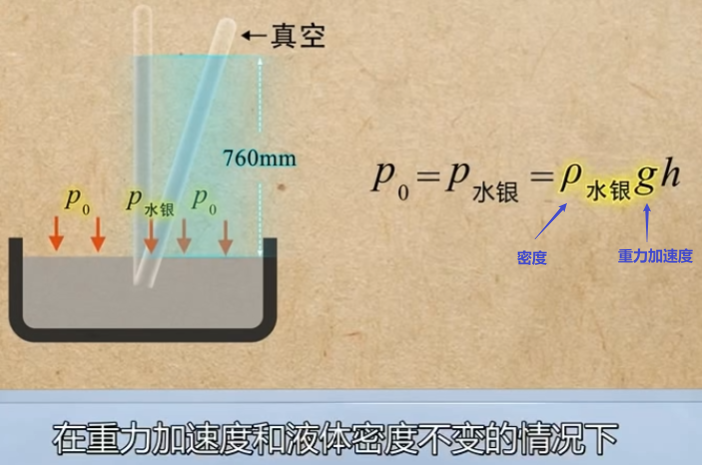
\includegraphics[width=0.3\textwidth]{img/0029.png} \\
	
	水银柱产生的压强 $p_{\text{水银}}=\text{标准大气压}p_0$, 根据压强公式 p=ρgh, 在水银密度ρ不变, 重力加速度g=9.8N/kg, 标准大气压 $p_0$,  这三个变量都不变的情况下, 显然水银柱的高度h 就不会改变.
	
	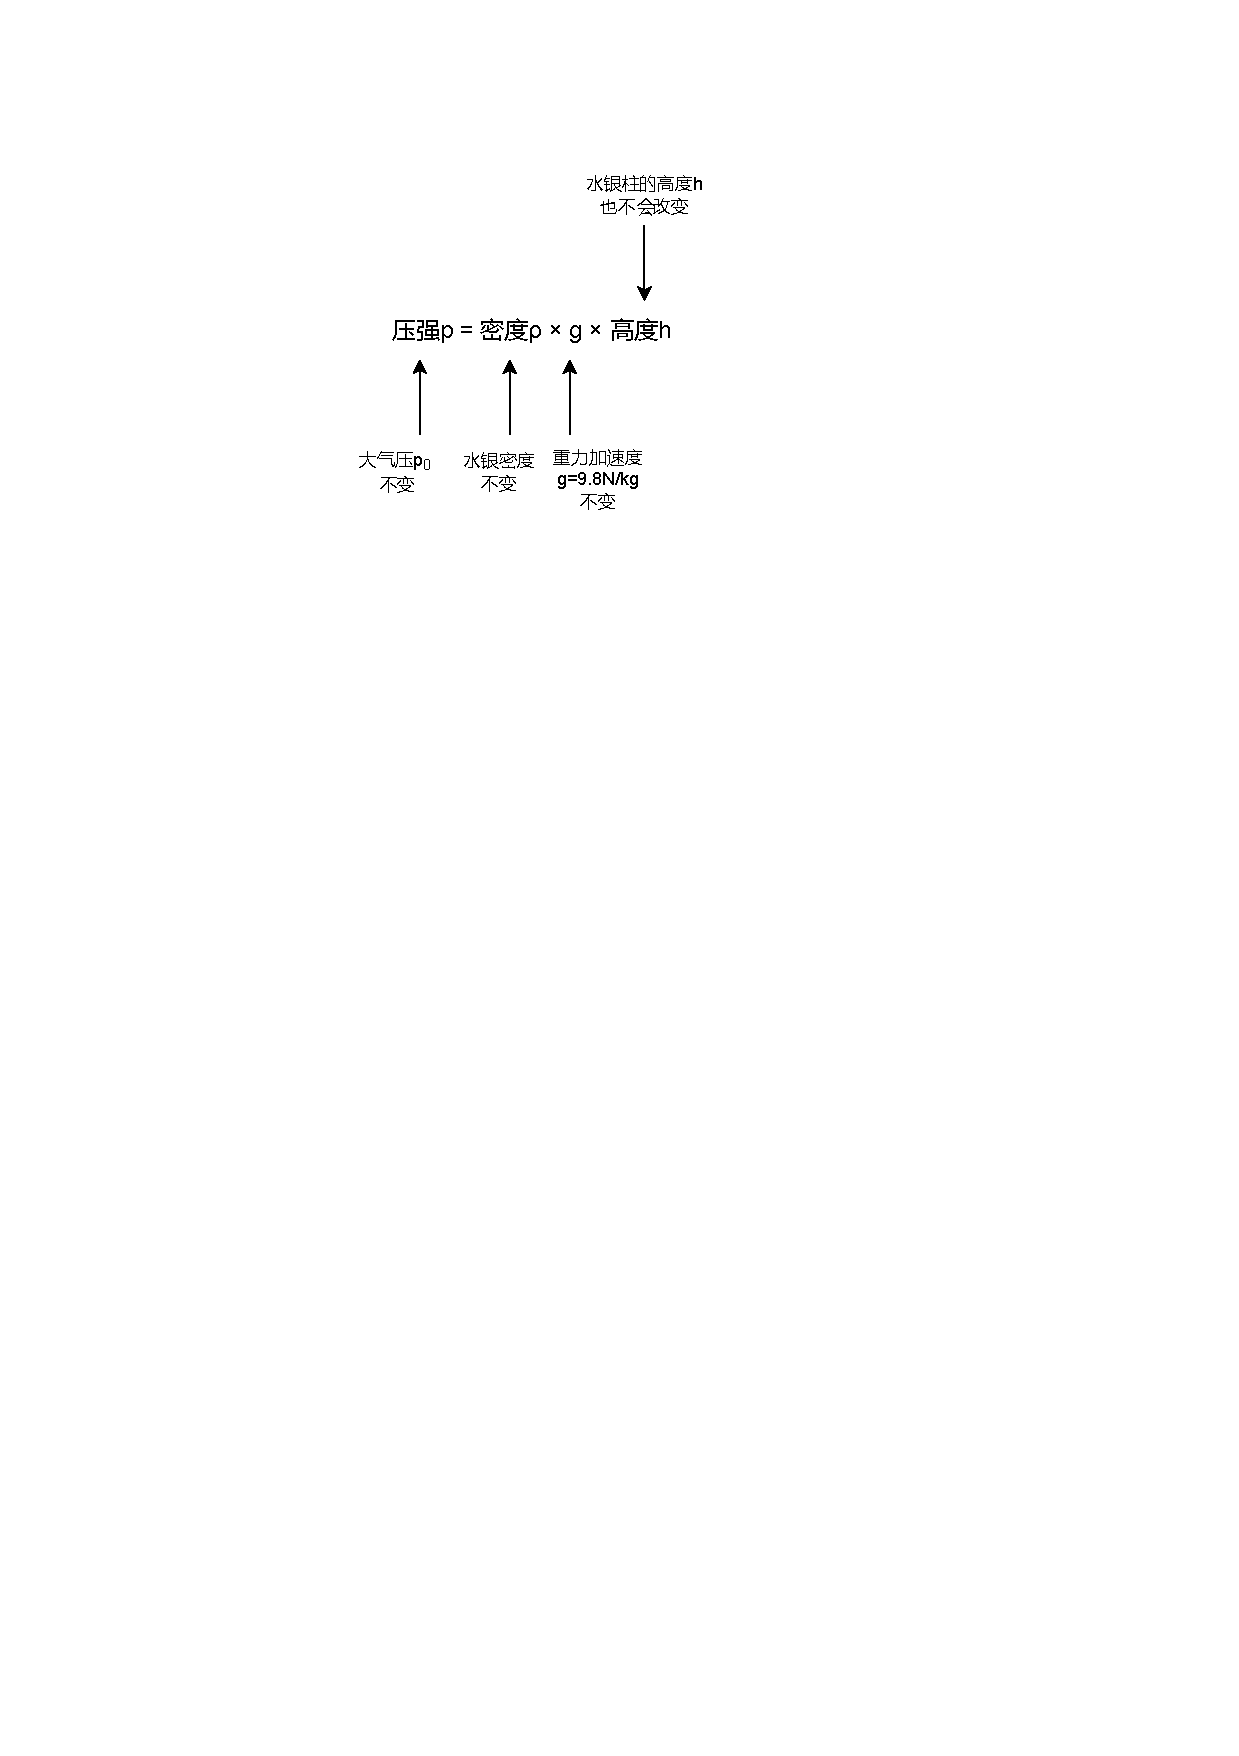
\includegraphics[width=0.3\textwidth]{img/0031.pdf} 
	
	同时这也说明, 某液体或气体深处的压力的大小, 跟其质量m的多少无关. 即使水银柱倾斜过来, 水银柱中水银的体积增加, 质量m增加, 它的压强p也不会改变. \\
	
	注意:只有在水银柱上部的空间是``真空"时, 水银柱的压强才跟大气压强相等. 如果水银柱上方不是真空, 而是混有空气, 则这段空间的气体, 也会对水银柱产生压强. 在这种情况下, 就是这个压强与水银柱产生的压强之和, 才等于大气压强.
	
	即: 管内水银柱的高度, 只随外界大气压的变化而变化, 而和管子的粗细、倾斜角度、管的长度, 及将玻璃管提起还是下压等因素无关. 只与水银柱的竖直高度有关. \\
	
	注意: 大气的密度是变化的, 在地面附近, 空气的密度较大, 随高度的增加, 空气的密度越来越小. \\
	
	所以, \textbf{在地表的大气压下, 压得水银柱高度为760 mm. 反过来说, 我们就把这样大小的大气压, 叫做``标准大气压" $p_0$.}
	
	\begin{align*}
		\boxed{
			\underset{\text{标准大气压}}{\underbrace{p_0}}=\underset{\text{水银密度}13.59g/cm³}{\underbrace{\rho }}\cdot \underset{9.8N/kg}{\underbrace{g}}\cdot \underset{0.76m}{\underbrace{h}}=1.013\cdot 10^5\ P_a			
		}
	\end{align*}
	
	水银的密度, 是水的密度的13.6倍. 
	
	\textbf{在粗略计算中, 标准大气压可以取为 $1×10^5 Pa$.}
		
	\vspace{1em} 
	
	
	
	\subsection{``标准大气压"下的水柱的高度是 10.336米}
	
	如果玻璃管中装的是水呢?	
	\begin{align*}  % 支持每行编号. 若不需要编号, 就用 align*环境
	& \underset{\text{标准大气压}}{\underbrace{p_0}}=p_{\text{水银}}=p_{\text{水}}\\
	& \text{即:\ }\underset{\text{水银密度}13.59g/cm³}{\underbrace{\rho }}\cdot \underset{9.8N/kg}{\underbrace{g}}\cdot \underset{0.76m}{\underbrace{h}}=\underset{\text{水的密度1.0\ }kg/m³}{\underbrace{\rho }}\cdot \underset{9.8N/kg}{\underbrace{g}}\cdot \underset{\text{水柱的高度}}{\underbrace{h}}\\
	& \text{最终会得到\ }h_{\text{水}}=10.336m\\ 
	\end{align*}
		
	\vspace{1em} 
	
	
	
	\subsection{(1)高度越高, 空气密度越小, 气压就越低. (2)气压越低, 沸点也就越低}
	
	从气压公式也可知道: \textbf{随着高度的升高(即 深度h 的减少. 你只需把空气想象成大海, 越接近地表的空气, 就如同海底的深度一样, 深度最大. 即 h最大. 这样, 随着海拔的增加, 越往天上去, 空气的深度h就越小, 气压就越小).}  换种说法就是: 海拔升高, 空气就越稀薄, 密度越小, 所以大气压会减小. 瓶中的空气的气压值超过了外面的气压, 就会将瓶中的水挤压到玻璃管中,  水柱的高度就会逐渐升高。
	
	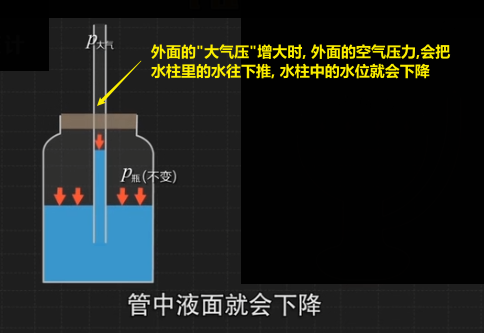
\includegraphics[width=0.45\textwidth]{img/0032.png} 
	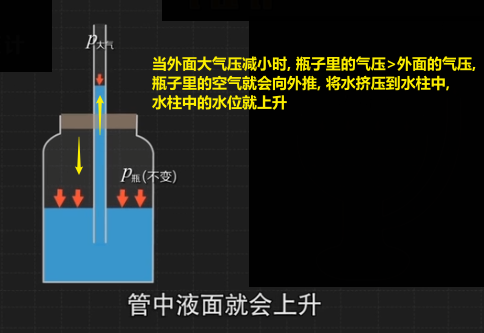
\includegraphics[width=0.45\textwidth]{img/0033.png} 
	
	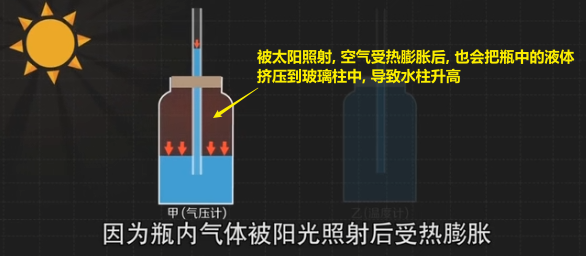
\includegraphics[width=0.45\textwidth]{img/0036.png} 	
	
	在海拔3000m 以内, 大约每升高10m, 大气压减小100 Pa. \\
	
	液体的沸点跟外部压强有关。当液体所受的压强(比如气压)增大时, 沸点也升高; 压强减小时,沸点也降低.   \\	
	- 蒸汽锅炉里的蒸汽压强, 约有几十个大气压, 锅炉里的水的沸点可在200℃以上. \\	
	- 在高山上煮饭, 比如青藏高原, 水的沸点仅为 84-87℃, 水就沸腾了, 但饭不易熟. 所以必须使用压力锅做饭, 以增强压力, 让沸点升高.
	
	
	
	
	
	
	
	\vspace{1em} 
	
	\subsection{自制气压计: 瓶中必须存在空气, 才能有气压, 才能在瓶中内外造成气压差.}
	
	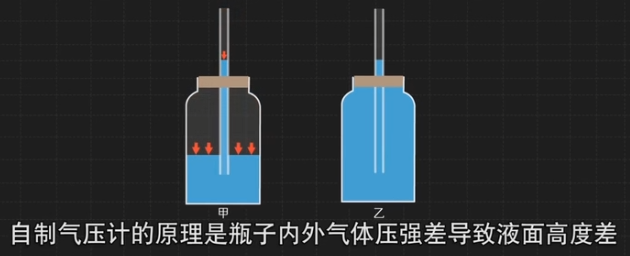
\includegraphics[width=0.45\textwidth]{img/0034.png} 
	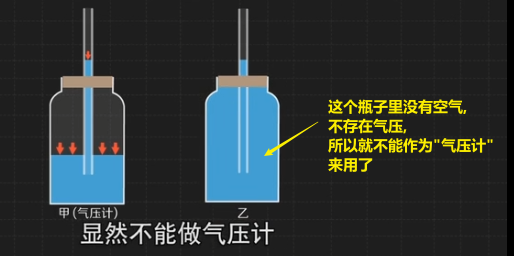
\includegraphics[width=0.45\textwidth]{img/0035.png} 
		
	
	~\\
	\hrule
	~\\
	
	
	\subsection{流体压强 : 流速越大的位置, 压强越小}
	
	\begin{tcolorbox}[title = {例},boxrule={0.1em},colframe={black!10}, colback={black!3},colbacktitle={black!10},coltitle={black}]
	两张垂落的纸, 向中间吹气, 纸张不会向外扬起, 而是向内靠拢. \\

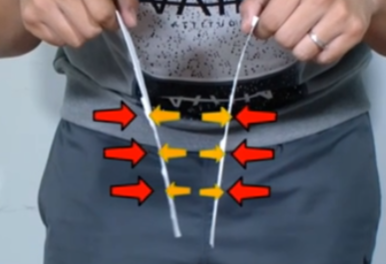
\includegraphics[width=0.45\textwidth]{img/0037.png}
	\end{tcolorbox}

	
	\begin{tcolorbox}[title = {例},boxrule={0.1em},colframe={black!10}, colback={black!3},colbacktitle={black!10},coltitle={black}]
	用纸做一个桥, 向桥洞里吹气, 桥会塌掉. \\


\includegraphics[width=0.45\textwidth]{img/0038.png} 	
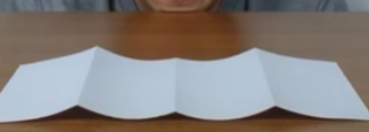
\includegraphics[width=0.45\textwidth]{img/0039.png} 
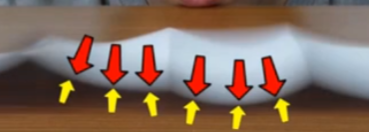
\includegraphics[width=0.45\textwidth]{img/0040.png} 
	\end{tcolorbox}


	
	上面这些现象, 是因为: \textbf{在气体和液体中, 流速越大的位置, 压强越小.} (吹气, 增大了流速).
	
	
	\begin{tcolorbox}[title = {例},boxrule={0.1em},colframe={black!10}, colback={black!3},colbacktitle={black!10},coltitle={black}]
		飞机为什么能够在空中飞行? 原因在于机翼的形状. \\
		
	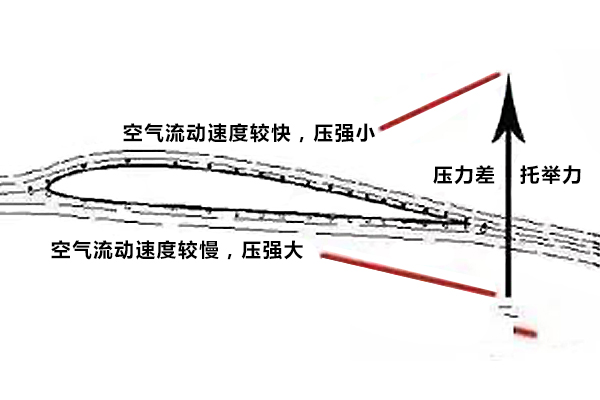
\includegraphics[width=0.45\textwidth]{img/0041.png}
	
	气流被机翼分成上、下两部分, 由于机翼横截面的形状上、下不对称, \textbf{在相同时间内,机翼上方气流通过的路程较长, 因而速度较大, 它对机翼上表面的压强较小; 而下方气流通过的路程较短, 速度较小, 它对机翼下表面的压强较大. 这样, 机翼上、下表面就存在着压强差, }因而有压力差, 这就是产生升力的原因.			
	\end{tcolorbox}



	\begin{tcolorbox}[title = {例},boxrule={0.1em},colframe={black!10}, colback={black!3},colbacktitle={black!10},coltitle={black}]
	火车站, 地铁站的站台上, 有一条安全线, 人必须站在安全线以外的区域. 否则, 当列车驶过时, 人站在安全线以内是非常危险的. 原因就在于列车速度造成的气压差, 会把你推向列车. \\
	
	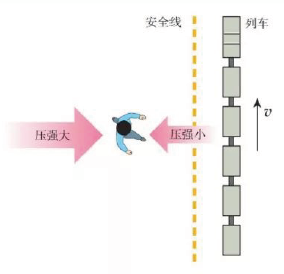
\includegraphics[width=0.45\textwidth]{img/0042.png} 
	\end{tcolorbox}


其他例子还有: 

- 风沿着窗外的墙面吹过时, 窗口悬挂的窗帘会飘向窗外. 即室内气压, 大于室外气压. 室内气压把窗帘往外推.


~\\
\hrule
~\\



\section{物体所受的浮力 buoyancy force = 该物体排开的液体或气体的重力G}

物体浸在液体中的体积越大(即物体排开的液体的体积越大)、\textbf{液体的密度越大, 则该物体受到的浮力就越大.} \\

阿基米德原理: 大量的实验结果表明, \textbf{浸在液体中的物体受到向上的浮力, 浮力的大小, 等于它排开的液体所受的重力.} 即:
\begin{align*}
	\boxed{
	F_{\text{浮力}}=G_{\text{排开的液体或气体的重力}}	
	}
\end{align*}

阿基米德原理, 不仅适用于液体, 也适用于气体.



\begin{tcolorbox}[title = {例},boxrule={0.1em},colframe={black!10}, colback={black!3},colbacktitle={black!10},coltitle={black}]
有一个重7N 的铁球, 当它浸没在水中时, 受到多大的浮力? 

根据公式: $F_{\text{浮力}}=G_{\text{排开的液体或气体的重力}}$ \\
我们知道了 $G_{\text{排开的液体或气体的重力}}$, 也就知道了浮力. \\

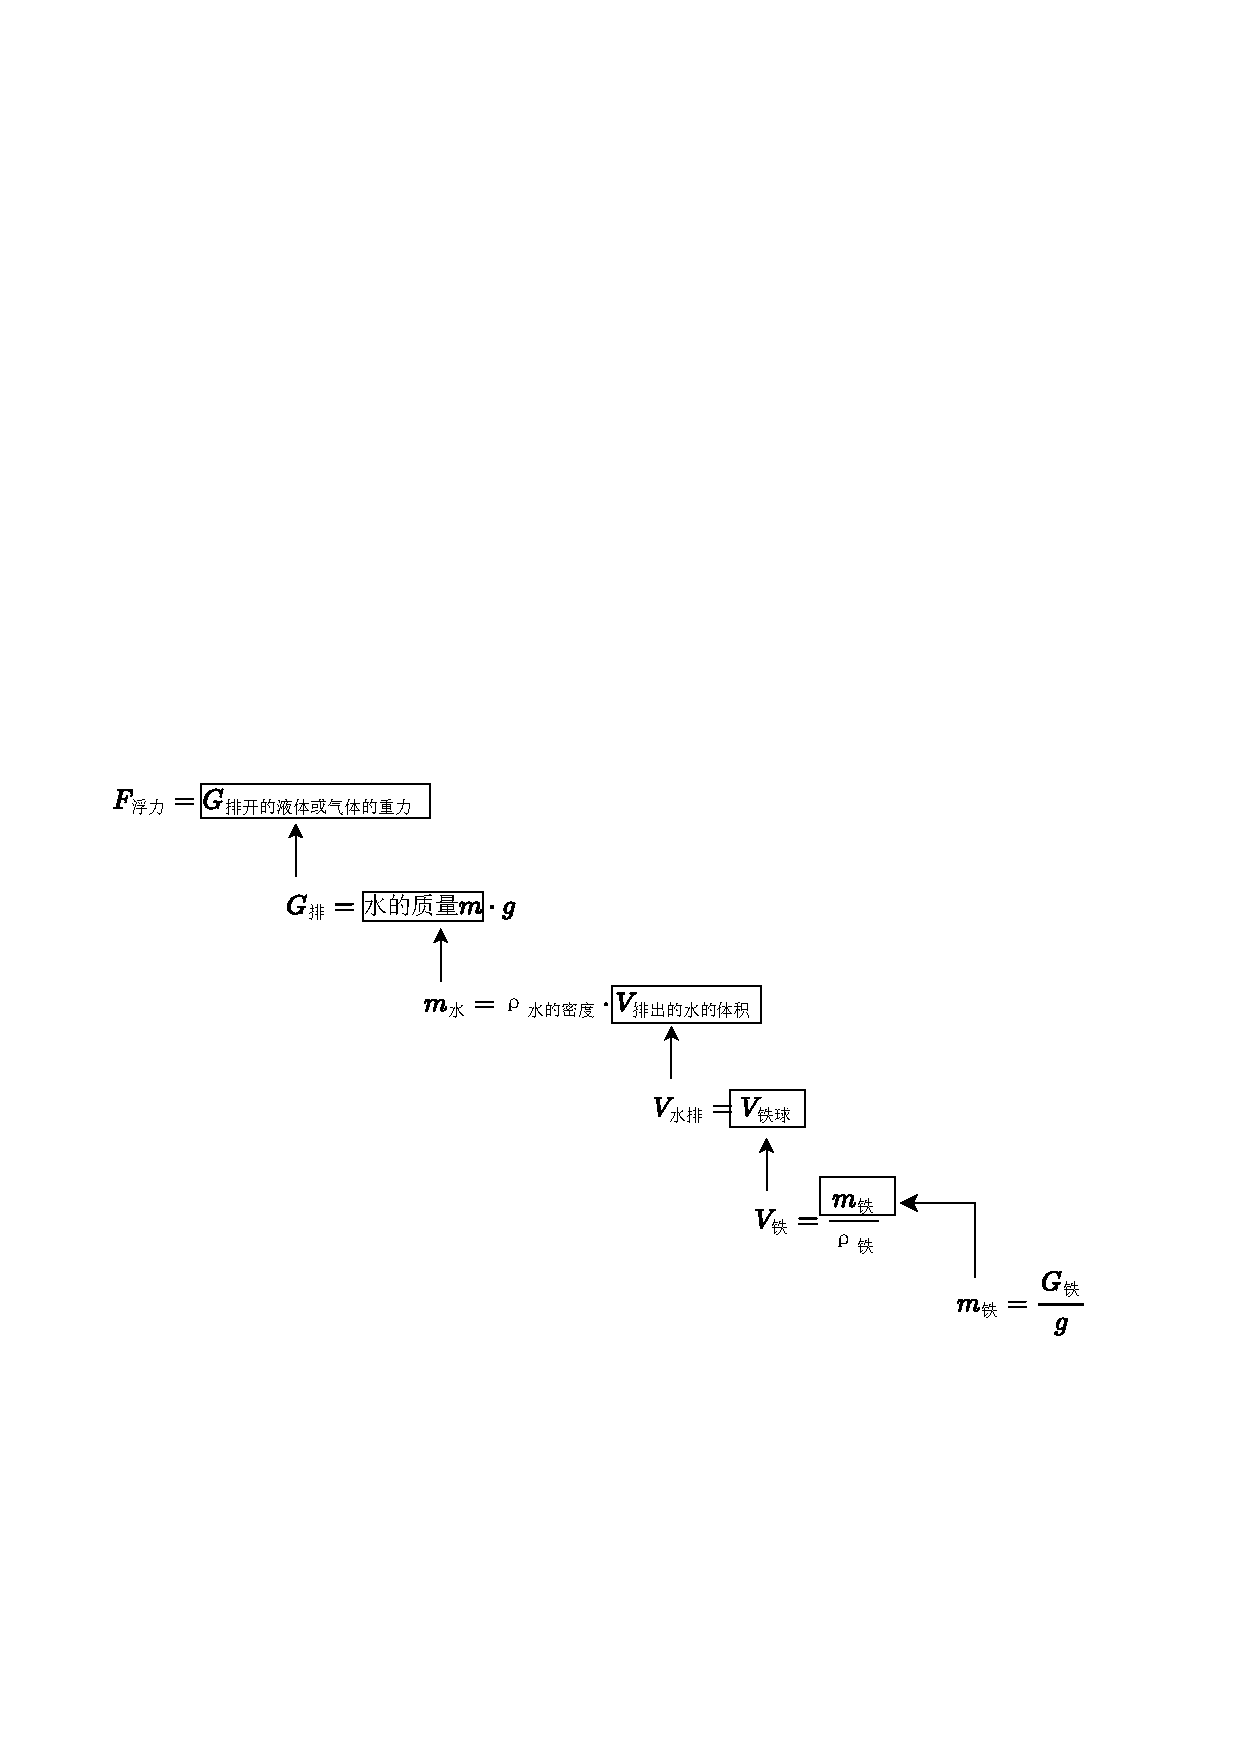
\includegraphics[width=1\textwidth]{img/0043.pdf}

根据上图的公式链, 我们从下往上来一步步求出每一个变量值. 
\begin{align*}
		& (1)\ m_{\text{铁}}=\frac{G_{\text{铁}}}{g}=\frac{7N}{9.8N/kg}=0.714286kg\\
	& (2)\ V_{\text{铁}}=\frac{m_{\text{铁}}}{\rho _{\text{铁的密度}}}=\frac{0.714286\ kg}{7.86\cdot 10^3kg/m^3}=9.08761\times 10^{-5}\ m^3\\
	& \left( 3 \right) \ V_{\text{水排}}=V_{\text{铁}}=9.08761\times 10^{-5}\ m^3\\
	& (4)\ G_{\text{水排}}=m_{\text{水}}g=\rho _{\text{水}}V_{\text{水排}}\cdot g=\left( 1\cdot 10^3kg/m^3 \right) \cdot \left( 9.08761\times 10^{-5}\ m^3 \right) \cdot 9.8N/kg=0.890586N\\
	& \left( 5 \right) \ F_{\text{浮力}}=G_{\text{排开的液体或气体}},\ \text{即}7N\text{重的铁球浮力是}0.89N\\	
\end{align*}

\end{tcolorbox}


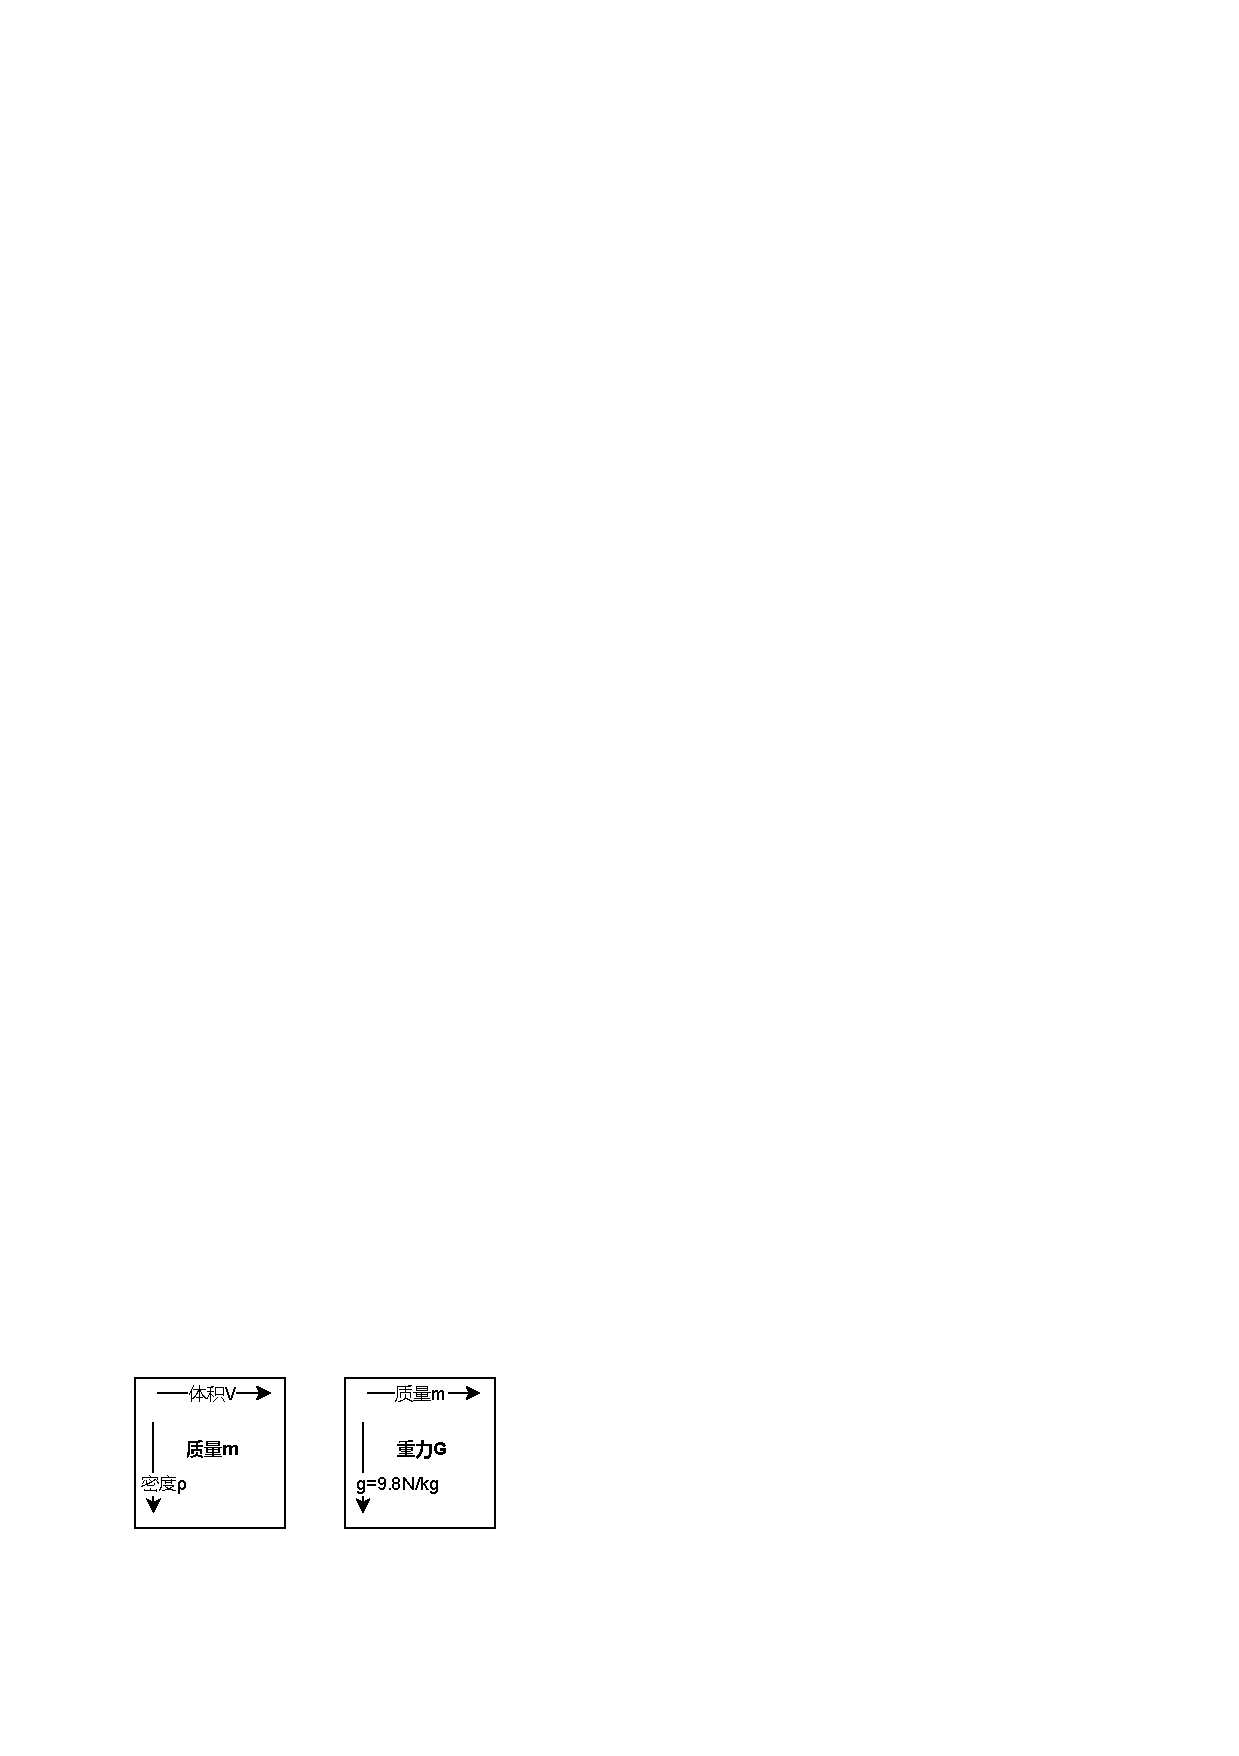
\includegraphics[width=0.4\textwidth]{img/0044.pdf}

浸没在液体中的物体: \\
→ 如果它的密度 < 液体的密度, 物体上浮;  \\
→ 如果它的密度 = 液体的密度, 物体可以悬浮在液体内任何地方; \\
→ 如果它的密度 > 液体的密度, 物体下沉. \\

\begin{tcolorbox}[title = {例},boxrule={0.1em},colframe={black!10}, colback={black!3},colbacktitle={black!10},coltitle={black}]
橡皮泥的密度, 大于水, 所以它在水中会下沉. 但如果把橡皮泥捏成瓢状, 放在水面, \textbf{虽然它的重力G 没有改变, 但是排开的水较多, 根据浮力公式}:  	
\begin{align*}
	\boxed{	
	F_{\text{浮力}}=G_{\text{排出的水的重力}}=m_{\text{水}}\cdot g=\left( \rho _{\text{水的密度}}\cdot V_{\text{排出的水的体积}} \right) \cdot g
	}
\end{align*}

\textbf{排开的水的体积变大, 浮力就也同比增加.} 所以橡皮泥船就能漂浮在水面上了. 钢铁轮船能浮在水上, 就是根据这个原理制造的. 
\end{tcolorbox}

轮船的大小, 通常用``排水量"来表示。排水量就是轮船``装满货物"时, 排开水的质量。如一艘轮船, 它的排水量是 $1×10^4 t$, 就是说此船在满载时, 货物质量和船身质量之和, 为$1×10^4 t$.



~\\
\hrule
~\\

\section{功 work = 力F × 移动距离s}

功 work: 如果一个力作用在物体上, 物体在这个力的方向上, 移动了一段距离, 就说这个力对物体做了``功".

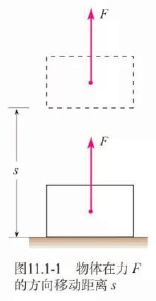
\includegraphics[width=0.2\textwidth]{img/0045.png}

\textbf{力学里所说的做功, 包含两个必要因素: (1) 作用在物体上的力, (2) 物体在这个力的方向上移动的距离.}

例如, 如果你搬一块石头而没有搬动, 虽然你对该物体施加了力, 但石头在力的方向上没有移动, 则你对该石头依然没有"做功". \\

力学中, 功 = 力 × 物体在力的方向上移动的距离. \\
所以, 作用在物体上的力越大, 物体在力的方向上移动的距离越大, 力所做的``功"也就越多. \\

公式即:
\begin{align*}
	\boxed{
		\underset{\text{功:单位焦耳}J}{\underbrace{W}}=\underset{\text{力:单位牛}N}{\underbrace{F}}\cdot \underset{\text{沿着力的方向移动的距离,单位:米}}{\underbrace{s}}		
	}
\end{align*}

功的单位, 是牛米. 它有一个专门的名称 -- 焦耳(joule), 简称焦, 符号是J. \\



\begin{tcolorbox}[title = {例},boxrule={0.1em},colframe={black!10}, colback={black!3},colbacktitle={black!10},coltitle={black}]
雪橇的质量m=50kg, 上装载木头350kg, 马拉雪橇匀速前进(雪橇受到的摩擦力是800N), 到3km外的目的地. 问马做了多少功? \\
既然马在匀速前行, 说明马的拉力F, 与摩擦力$F_摩$大小相等.

$
\text{功}Work=F_{\text{马的拉力}}\cdot s=F_{\text{雪橇受到的摩擦力}}\cdot s=800N\cdot 3000m=2.4\times 10^6J
$
\end{tcolorbox}
	
	\vspace{1em} 
	
	
	
\subsection{$\text{功率}Power=\frac{\text{功}Work}{\text{时间}time}$ }	

A和B做相同的``功",  完成时间短的, ``做功"快. \\
相同时间内, ``做功"多的那个物体, ``做功"快. \\
	
就像用速度表示运动的快慢一样, 在物理学中, \textbf{用``功率"表示做功的快慢. ``功"与``时间"之比, 叫做功率(power).} 公式即:
\begin{align}
	\boxed{
	\underset{\text{功率,单位:瓦特}Watt}{\underbrace{Power}}=\frac{\underset{\text{功,单位:焦耳}}{\underbrace{Work}}}{\underset{\text{时间,单位:秒}}{\underbrace{time}}}		
	}
\end{align}

- 功: 单位是``焦耳" \\
- 时间 : 单位是``秒" \\
- 功率 : 单位是``焦耳每秒", 它有个专门的名称叫``瓦特"(watt), 简称瓦, 符号是W. 功率还有个常用单位是: 千瓦(kW). \\
\begin{align*}
	\boxed{
	1kW = 10^3 W
	}
\end{align*}

\textbf{功率在数值上, 等于单位时间内所做的功.}



\begin{tcolorbox}[title = {例},boxrule={0.1em},colframe={black!10}, colback={black!3},colbacktitle={black!10},coltitle={black}]
	一块石头的质量m=6t, 起重机在15秒内, 将该石头垂直匀速提升了1m, 则该起重器的功率是多少? \\
	
	既然是匀速提升, 则起重机的拉力, 与石头所受的重力相等.	
	\begin{align*}
			&\text{功率}Power=\frac{\text{功}Work}{\text{时间}time}\\
		&=\frac{\text{拉力}F\cdot \text{移动距离}s}{t}=\frac{\overset{=\text{起重机拉力}F}{\overbrace{\text{石头的重力}G}}\cdot s}{t}\\
		&=\frac{\left( m_{\text{石头}}g \right) \cdot s}{t}=\frac{6000kg\cdot 9.8<\frac{N}{kg}>\cdot 1<m>}{15<s>}=3920<Watt>\\		
	\end{align*}
\end{tcolorbox}


	\vspace{1em} 
	

	
	\subsection{动能}
	
	流水, 能推动水车. 子弹, 能击穿靶体. 流水、子弹都做了``功".  \textbf{物体能够对外``做功", 我们就说这个物体具有``能量"(energy), }简称能. \\
	``能量"的单位, 与``功"的单位相同, 也是``焦耳".
	
	\textbf{一个物体能够做的``功"越多、表示这个物体的``能量"越大.} \\
	
	运动的钢球打在木块上,木块被推走, 钢球对木块做了功。\textbf{钢球能够做功,表明钢球具有能量。}
	
	\textbf{物体由于运动而具有的能, 叫做动能(kinetic energy).} 一切运动的物体都具有动能. \\
	
	kinetic: adj.  /kɪˈnetɪk/  ( technical 术语) of or produced by movement 运动的;运动引起的. kinetic energy 动能 \\
	
	
	动能的大小跟哪些因素有关呢?
	→ 质量m 相同的物体, \textbf{运动的速度越大, 它的动能越大} \\
	→ 运动速度相同的物体, \textbf{质量越大, 它的动能也越大} \\
	
	
\begin{tcolorbox}[title = {例},boxrule={0.1em},colframe={black!10}, colback={black!3},colbacktitle={black!10},coltitle={black}]
某道路路标显示: 小型客车最高行驶速度不得超过100 km/h. 大型客车、载货汽车最高行驶速度不得超过80 km/h. 限速之差, 正是考虑到动能值的问题.  大车比小车质量大, 如果它们速度相同, 大车的``动能"会大于小车的动能. 因此, 要对不同质量的车型, 限定不同的最高行使速度.
\end{tcolorbox}
	
	\vspace{1em} 
	
	
	\subsection{势能 potential energy}
	
	重力势能: 打桩机, 把重锤高高举起, 重锤落下, 可以把桩打入地里, 重锤对桩做了功。高处物体所具有的能, 叫做``重力势能". \textbf{物体的质量越大,位置越高,它具有的``重力势能"就越大.	} \\
	
	弹性势能: 拉弯的弓能将箭射出, 具有能量. 这是因为发生形变的物体, 在恢复形变时, 可以做功, 因此具有能量.  \\
	物体由于发生``弹性形变", 而具有的能, 叫做``弹性势能". \textbf{物体的弹性形变越大, 它具有的``弹性势能"就越大.}
	
	
	\vspace{1em} 
	
	
	
	\subsection{机械能 = 动能 + 势能}
	
	- 一个物体从高处下落, 物体的``重力势能", 转化成了它的``动能". \\
	- 弯弓射箭时, 弓的``弹性势能", 转化成箭的``动能". \\
	- 蹦床运动员从高处落下, 在与蹦床面将要接触时,具有一定的动能. 与蹦床面接触后, 床面发生弹性形变, 运动员的``动能", 转化成蹦床的``弹性势能". \\
	可见, \textbf{``动能"和``势能"可以相互转化.} \\
	
	\begin{tcolorbox}[title = {例},boxrule={0.1em},colframe={black!10}, colback={black!3},colbacktitle={black!10},coltitle={black}]
	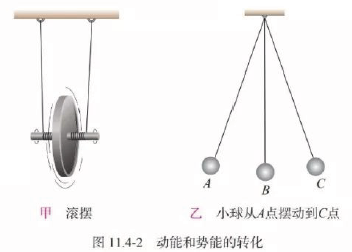
\includegraphics[width=0.4\textwidth]{img/0046.png}
	
	- 上图, 滚摆下降时, 它的``重力势能"越来越小, ``动能"越来越大, 重力势能转化为动能。滚摆上升时, 它的``动能"越来越小, ``重力势能"越来越大, 动能转化为重力势能.
	
	- 上图, \textbf{小球从A点下落到B点, ``重力势能"逐渐转化成``动能", 到最低点B时``动能"最大.} 之后又从B点上升到C点, 动能逐渐转化成重力势能.	
	\end{tcolorbox}

	大量研究结果表明, \textbf{如果只有``动能"和``势能"来相互转化的话(即不考虑阻力), 尽管动能、势能的大小会变化, 但``机械能"的总和不变. 即: 机械能是``守恒"的.} \\
	
	
	机械能(Mechanical energy), 就是``动能"与``势能"的总和. 这里的``势能", 分为``重力势能"和``弹性势能".  \\
	→ \textbf{决定``动能"的, 是质量, 与速度.} \\
	→ \textbf{决定``重力势能"的, 是质量, 和高度.} \\
	→ \textbf{决定``弹性势能"的, 是劲度系数, 与形变量.} \\
	
	机械能, 是表示物体``运动状态"与``高度"的物理量. \\
	运动状态, 是指物体进行``机械运动"时, 相对某个``参考系"的状态。``运动状态"有: 静止、匀速运动、加速运动、减速运动, 也有直线运动、曲线运动等多种状态。 \\
	
	
	
	\begin{tcolorbox}[title = {例},boxrule={0.1em},colframe={black!10}, colback={black!3},colbacktitle={black!10},coltitle={black}]
把一个吊起来的铁物, 从你鼻子附近放手, 让它摆来摆去. 想想看, 铁物摆回来时, 会打到你的鼻子吗?

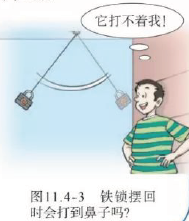
\includegraphics[width=0.25\textwidth]{img/0047.png}
	\end{tcolorbox}
	
	
	
	~\\
	\hrule
	~\\
	
	
	\section{简单机械}






	
	\subsection{杠杆 lever}
	
	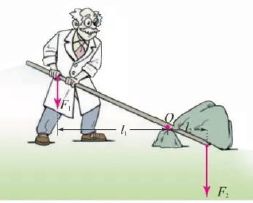
\includegraphics[width=0.4\textwidth]{img/0048.png}
	
	
	杠杆的平衡条件是: 动力×动力臂 = 阻力×阻力臂	
	\begin{align}
		\boxed{
			F_{\text{动力}}\cdot l_{\text{动力臂}}=F_{\text{阻力}}\cdot l_{\text{阻力臂}}			
		}
	\end{align}
	
	
	
	\begin{tcolorbox}[title = {例},boxrule={0.1em},colframe={black!10}, colback={black!3},colbacktitle={black!10},coltitle={black}]
	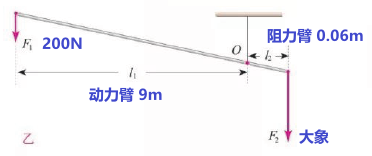
\includegraphics[width=0.4\textwidth]{img/0049.png}	
	\begin{align*}
			& \text{根据公式:\ }\underset{200N}{\underbrace{F_1}}\underset{9m}{\underbrace{l_1}}=\underset{=G_{\text{大象的重力}}}{\underbrace{F_2}}\underset{0.06m}{\underbrace{l_2}}\\
		& F_2=\frac{200\cdot 9}{0.06}=30000N=G_{\text{大象的重力}}=m_{\text{大象的质量}}g\\
		& m_{\text{大象的质量}}=\frac{G_{\text{大象的重力}}}{g}=\frac{30000N}{9.8N/kg}=3061.22kg\approx 3t\\		
	\end{align*}
	\end{tcolorbox}
	
	
	- 等臂杠杆: 动力臂长 = 阻力臂长 \\
	- 省力杠杆: 动力臂长 > 阻力臂长 \\
	- 费力杠杆: 动力臂长 < 阻力臂长 \\
	比如划船, 手移动较小的距离, 使船桨在水中移动较大的距离, 这就是``费力杠杆". 为了省距离, 而费了力气.
	
	
	\vspace{1em} 
	
	
	\subsection{滑轮 pulley}
	
	85
	
	
	~\\
	\hrule
	~\\
	
	\section{内能}
	
	\subsection{分子热运动}
	
	一切物质的分子, 都在不停地做无规则的运动。\textbf{温度越高, 分子运动越剧烈.} \\
	由于分子的运动跟温度有关, 所以这种无规则运动, 叫做分子的``热运动"(thermal motion). \\
	
	分子之间既有``引力"又有``斥力".
	
	气体分子之间的距离 >  液体分子之间的距离 > 固体分子之间的距离.
	
	\vspace{1em} 
	
	
	
	\subsection{内能 internal energy}
	
	【分子的动能】: \\	
	运动的物体具有``动能", 运动的分子也同样具有``动能". 分子在不停地做热运动, \textbf{温度越高, 分子``热运动"的速度越大, 动能也就越大。} \\	
	
	【分子的势能】: \\
	分子之间也具有相互作用力, 所以分子也具有``势能". \\
		
	【物体的内能】: \\
	\textbf{一个物体的所有分子的动能 + 势能 = 该物体的``内能".}  \\
	
	
	【``内能"的单位】: 是焦耳(J). 各种形式能量的单位, 都是焦耳. \\
	
	【内能和温度有关】: \\
	→ \textbf{物体温度升高时, 内能增加.}  \\
	→ \textbf{温度下降时, 内能减少.} \\
	
	【热传递, 可以改变物体的``内能"】: \\
	把一个热的东西放到冷水中, 东西会冷下来, 而冷水会变热. 这是因为在此过程中发生了``热传递"。 \\
	发生热传递时, 高温物体``内能"减少, 低温物体``内能"增加。 \\
	
	在热传递过程中,\textbf{传递能量的多少, 叫做``热量"( quantity of heat), 热量的单位也是焦耳。} \\
	\textbf{物体吸收热量时, 内能增加; 放出热量时, 内能减少。}物体吸收或放出的热量越多, 它的内能改变越大。 \\
		
		
	【做功, 能改变物体的``内能"】: \\
	→ 外界, 对系统做功, 系统内能增加. \\
	→ 系统, 对外界做功, 系统内能减少 \\
	
	\begin{tcolorbox}[title = {例},boxrule={0.1em},colframe={black!10}, colback={black!3},colbacktitle={black!10},coltitle={black}]
	对瓶中的空气做压缩时, 外界对空气做功, 根据能量守恒定律, 内能增加, 所以温度升高. \\
	拿掉塞子后, 瓶中的压缩气体开始膨胀, 对外做功, 瓶内空气内能减小, 温度降低, 所以瓶中的水蒸气就冷却液化, 变成小水滴(即白雾).
	\end{tcolorbox}
	
	
\vspace{1em} 



\subsection{比热容}

质量m 相同的两种不同物质A和B, 使它们升高相同的温度, 在此过程中, 它们吸收热量的多少, 是不同的. \\




【比热容, 比热容量】: \\
Specific Heat Capacity. 简写为C. 就是\textbf{用来衡量: 1单位质量的某种物质, 在升高(或下降) 1单位温度时, 所吸收(或放出)的热量.}  \\
注意: 它衡量的是, 物质提高温度时所需热量的能力, 而不是它吸收或散热的能力. \\

下面的公式用来表明: m质量物体的温度要变化1度, 需要多少热量?
\begin{align*}
	\boxed{
		\text{质量为}m\text{的物体,其热容量}C=\frac{\varDelta \text{热量的变化量}}{\varDelta \text{温度的变化量}}
	}
\end{align*}  

下面的公式的意思就是:1单位质量的物体要变化1度, 需要吸收或释放多少热量?
\begin{align*}
	\boxed{
		\text{比热容}c=\frac{\text{热容量}C}{\text{质量}m}=\frac{\varDelta \text{热量的变化量}}{\text{质量}m\cdot \varDelta \text{温度的变化量}}		
	}
\end{align*} \\



【比热容的单位】: 焦耳/每千克摄氏度. 即令1kg的物质的温度上升1摄氏度时, 所需吸收(或释放)的热量. 符号是 J/(kg·℃) \\


【比热容的值】: \\
\textbf{单位质量的某种物质, 温度降低1℃时所放出的热量, 与它温度升高1℃时所吸收的热量, 相等. 数值上也等于它的比热容.} \\

``比热容"是反映物质自身性质的物理量。不同的物质, 比热容一般不同. \\

- 水的比热容: $4.2 \cdot 10^3$  J/(kg·℃). 即1千克的水, 温度升高(或降低)1摄氏度时, 所吸收(或放出)的热量为4200J. \\
- 冰的比热容: $2.1 \cdot 10^3$  J/(kg·℃).  \\

质量相同的不同物质, \textbf{当吸收或放出同样热量时, ``比热容"较大的物质, 温度变化较小。 因此, 比热容大的物质, 对调节温度有很好的作用.} \\


\textbf{把物体的温度上升, 想象成"吃饱". 把物体吸收的热量, 想象成"饭量":} \\
→ \textbf{比热容大的物体, 就是饭量大, 他要吃很多饭量(吸收很多热量), 才能吃饱(自己温度上升1度).}  \\
→ \textbf{比热容小的物体, 就是饭量小, 他只吃一点点饭量(吸收很少的热量), 就吃饱了(自己温度上升1度).}  \\


水的比热容较大, 意味着当环境温度变化较快的时候, 水的温度变化相对较慢。\textbf{生物体内水的比例很高, 有助于调节生物体自身的温度, }以免温度变化太快对生物体造成严重损害。 \\


\begin{tcolorbox}[title = {例},boxrule={0.1em},colframe={black!10}, colback={black!3},colbacktitle={black!10},coltitle={black}]
水的比热容是沙石的4倍多, 这就意味着: \\
→ 海边的夏天, 尽海水吸收了许多热量, 但是由于它的比热容较大, 所以海水的温度变化并不大, 海边的气温变化也不会很大. \\
→ 而在沙漠, 由于沙石的比热容较小, 吸收同样的热量, 温度会上升很多. 所以沙漠的昼夜温差很大. 
\end{tcolorbox}


\vspace{1em} 


	
	\subsection{热机}
	
	【热机】: \\
	瓶中的水, 在被加热的过程中, 产生热量, 传给水和水蒸气; 塞子受到水蒸气的压力而冲出去. 即, 水蒸气的内能, 转化为了塞子的动能. 这就是蒸汽机的工作原理. \\	
	
	人们发现``内能"可以``做功", 就制造了各种\textbf{利用``内能"做功的机械——热机(heat engine).} \\	
	热机的种类很多, 包括: 蒸汽机、内燃机、汽轮机、喷气发动机等. \\
	
	
	【内燃机】: \\
	燃料直接在发动机汽缸内燃烧产生动力的热机, 叫做内燃机. 如汽车. 内燃机分为汽油机和柴油机两大类. \\
	
	
	【热值 calorific value】: \\
	燃料有很多, 包括: 木柴, 煤, 汽油, 酒精, 煤气, 天然气等. 但是相同质量的不同燃料, 燃烧时所放出的热量是不相同的. 例如, 燃烧 1kg煤 放出的热量, 是燃烧 1kg 木柴放出热量的两倍多. \\
	
	热值: 我们\textbf{把某种燃料, 完全燃烧放出的热量, 与其质量之比, 叫做这种燃料的``热值". 热值 = 1kg某种燃料完全燃烧放出的热量.} \\
	在食品化学中, ``热值"表示食物能量的指标. 指1g食物在体内氧化时所放出的热量. \\
	
	``热值"的单位,  由热量的单位和质量的单位组合而成. 在国际单位制中, 热量的单位是焦耳, 质量的单位是千克, 则\textbf{``热值"的单位是: ``焦/每千克", 符号是 J/kg.} \\
	常用的热值单位, 是: J/kg (固体燃料和液体燃料), 或J/m³ (气体燃料). \\
	
	
	根据燃料的``热值", 我们能计算出燃料完全燃烧时放出的热量: \\
	- 氢的热值: $1.4 \cdot 10^8$ J/kg \\
	- 汽油的热值: $4.6 \cdot 10^7$ J/kg \\
	- 柴油的热值: $4.3 \cdot 10^7$ J/kg \\
	- 煤气的热值: $3.9 \cdot 10^7 J/m^3$ \\
	
	
	
	【热机的效率】: \\
	我们很难利用燃料中蕴含的全部``热值", 原因是: \\
	- 燃料很难完全燃烧, 所以它放出的热量, 往往比按``热值"计算出的要小.  \\
	- 即使它释放出的那部分热量, 也无法全部被我们利用. 有一部分热量会直接散失掉. \\
	
	对于热机而言, 燃料释放的能量, 只有一部分能被用来做有用的功, 还有相当一部分能量散失掉了。\textbf{用来做有用``功"的那部分能量, 与燃料完全燃烧放出的``能量"之比, 叫做`热机的效率`"。} \\
	→ 蒸汽机的效率很低,只有6\%~15\%. 	\\
	→ 内燃机中, 由于燃料是在汽缸内部燃烧的, 而且燃料与空气混合充分, 燃烧得比较完全, 所以内燃机的效率比蒸汽机的高。但汽油机的效率也只有20\%-30\%; 柴油机的效率为30\%-45\%. \\
	
	所以, 热机的效率高, 就意味着在``做功"同样多的情况下, 消耗的燃料就更少. \\
	
	在热机的能量损失中, 废气带走的能量最多。 在热电站中, 人们利用蒸汽轮机排出的废气来供热. 来减少能量浪费. \\

	
	\vspace{1em} 
	
	
	\subsection{能量是能转化的 → 能量守恒定律}
	
	各种形式的能量, 是可以相互转化的: \\
	- 机械能 → 内能 : 摩擦生热 \\
	- 机械能 → 电能 : 水电站里水轮机, 带动发电机发电 \\
	- 电能 → 机械能 : 电动机带动水泵, 把水送到高处 \\
	- 光能 → 化学能 : 植物吸收太阳光进行光合作用 \\
	- 化学能 → 内能 : 燃料燃烧时发热 \\
	
	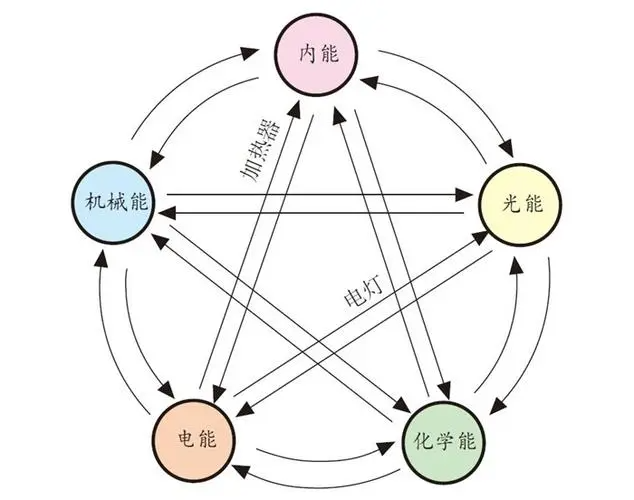
\includegraphics[width=0.4\textwidth]{img/0050.png} \\
	
	停止用力, 秋千会越摆越低; 掉在地上的弹性小球会跳起, 但是越跳越低。\textbf{在秋千和小球的运动中, 看似能量减少了, 其实是在运动过程中, 有一部分``机械能"转化成了``内能"。例如, 小球在跳动过程中会变热。} \\
	
	
	【能量守恒定律 law of conservation of energy】: \\
	\textbf{能量既不会凭空消灭, 也不会凭空产生, 它只会从一种形式, 转化为其他形式; 或者从一个物体, 转移到其他物体. 而在转化和转移的过程中, 能量的总量保持不变。这就是``能量守恒定律" law of conservation of energy.} \\
	
	例如, 在行驶的汽车中, 燃料的化学能, 通过燃烧转化为燃气的内能, 再通过热机做功, 把内能转化为机械能。在这个过程中, 燃料的化学能, 一部分转化为机械能, 一部分转化成了热机, 和周围环境的内能。 \\
	
	任何一部机器, 只能使能量, 从一种形式转化为另一种形式, 而不能无中生有地制造能量。因此, 根本不可能造出永动机.
	
	~\\
	\hrule
	~\\
	
	
	\section{电路}
	
	\subsection{电荷: 正电荷, 负电荷}
	
	自然界只有两种电荷: \\
	→ 正电荷 positive charge : 与用``丝绸"摩擦过的``玻璃棒"带的电荷相同. \\
	→ 负电荷 negative charge : 与用``毛皮"摩擦过的``橡胶棒"带的电荷相同. \\
	
	同种电荷互相排斥,异种电荷互相吸引。\\
	
	
	【电荷量】: \\	
	物体所带电荷的数量, 叫做电荷量。电荷量也可简称电荷。 \\
	\textbf{``电荷量"的单位是库仑(column)},简称库,符号是C。\\
	一根实验室中常用的玻璃棒或橡胶棒,摩擦后所带的电荷量, 大约只有 $10^{-7} C$. \\
	
	原子中, 在原子核周围,有一定数目的电子 electron 在核外运动。\textbf{电子是带有最小负电荷的粒子},所带电荷量为 $1.6 \cdot 10^{-19} C$. \\
	\textbf{而原子核, 带正电。\textbf{通常,原子核所带的正电荷, 与核外``所有电子"所带的负电荷, 在数量上相等. 因此原子整体上不显电性, 物体对外也不显电性。}} \\
	
	- 氢原子, 原子核中有1个正电荷(其电荷量, 与电子电荷量相等),核外有1个电子。 \\
	- 氦原子核中, 有2个正电荷,核外有2个电子。 \\
	
	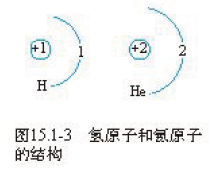
\includegraphics[width=0.25\textwidth]{img/0051.png} \\
	
	不同物质的原子核, 束缚电子的本领不同。\textbf{当两个物体摩擦时,哪个物体的原子核束缚``电子"的本领弱,它的一些电子就会转移到另一个物体上。} \\
	→ 失去电子的物体, 因为缺少电子, 而带正电. \\
	→ 得到电子的物体, 因为有了多余电子, 而带等量的负电。 \\
	所以, 摩擦起电并不是创造了电荷,而只是将电荷从一个物体转移到另一个物体. \\
	
	
	带电的物体有时会与其他的物体接触,从而失去电荷。那么,什么物体容易传导电荷, 什么物体不容易传导电荷呢? \\			
	→ 导体 conductor : 即容易导电的物体. 包括: 金属、人体、大地、石墨、食盐水溶液等. \\
	→ 绝缘体 insulator : 即不容易导电的物体. 包括: 橡胶、玻璃、塑料等. \\
	
	电荷在金属中可以定向移动,说明金属是可以导电的。 \textbf{在金属中,部分电子可以脱离原子核的束缚,而在金属内部自由移动, 这种电子叫做``自由电子"。金属导电,靠的就是自由电子。} \\	
	
	\vspace{1em} 
	
	
	\subsection{电流 : 流动方向从 正级 → 负级}
	
	\textbf{电荷虽然能在金属导体中, 做定向移动,但这种定向移动瞬间就结束了。 而生活中, 点亮的小灯泡能持续发光, 是因为有电荷持续不断地流过小灯泡。}那么怎样才能使电荷不断地流过小灯泡呢?  -- 必须要有电池 cell, 还要用导线将它们与电池连接成闭合的回路。	\\	

	导线、小灯泡的灯丝, 都是金属做的。\textbf{金属里面有大量自由电子,它们可以自由移动。平时金属内``自由电子"运动的方向杂乱无章, 但是接上电池之后, 它们就受到了推动力,就会做``定向移动". 电荷的定向移动, 就形成了``电流" electric current.} \\
	
	回路中有电流时, 发生定向移动的电荷, 可能是正电荷, 也可能是负电荷, 还有可能是正、负电荷同时向相反方向发生定向移动。在19世纪初,物理学家刚刚开始研究电流时,并不清楚在各种情况下, 究竞是哪种电荷在移动,当时就\textbf{把``正电荷定向移动的方向"规定为电流的方向。} \\
	按照这个规定, 当电池、导线、小灯泡组成的回路闭合时, 在电源外部,\textbf{电流的方向, 是从电源``正极"经过用电器, 流向``负极"的}。 \\
	
	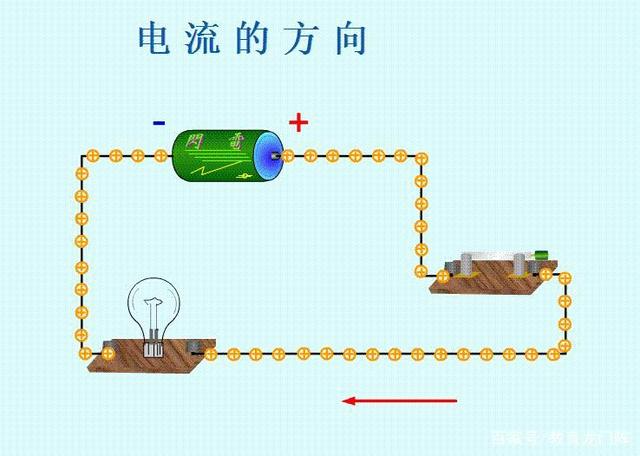
\includegraphics[width=0.4\textwidth]{img/0052.png} \\
	
	
	【通路】 : \\
	【断路】 : \\
	【短路】 : \\
	【短接】 : \\
	
	
	【串联】 : \\
	两个小灯泡依次相连, 然后接到电路中, 这两个小灯泡就是串联 series connection 的。 \\
	
	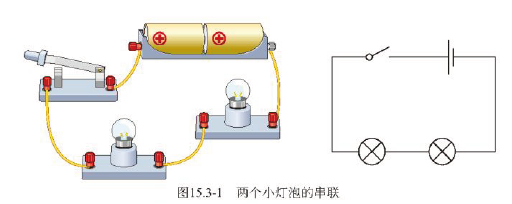
\includegraphics[width=0.4\textwidth]{img/0053.png} \\			
	
	【并联】 : \\
	两个小灯泡的两端分别连在一起,然后接到电路中, 这两个小灯泡是并联 parallel  connection 的。并联电路中两个用电器共用的那部分电路, 叫干路. 单独使用的那部分电路, 叫支路。 \\
	
	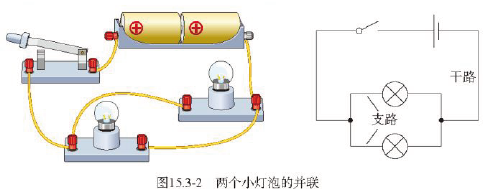
\includegraphics[width=0.4\textwidth]{img/0054.png} \\
	
	
	→ 在``串联"电路中, 开关可以控制所有用电器, 开关位置的改变并不影响它对用电器的控制作用。 \\
	→ 在``并联"电路中,干路开关, 可以控制所有用电器. 而\textbf{支路开关, 只能控制其所在支路的用电器。} \\
	家庭中的电灯、电吹风机、电冰箱、电视机、电脑等用电器, 大多是``并联"在电路中的。 \\	
	
	
\includegraphics[width=0.25\textwidth]{img/0055.png} \\	
	
	\vspace{1em} 
	
	
	\subsection{电流的强弱: 单位 安培 ampere}
	
	【电流的单位: 安培】 : \\
	表示电流强弱的物理量, 是电流 electric current ,通常用字母I表示. 它的单位是安培 ampere,简称安, 符号是A. \\
	
	其他单位还有: mA 毫安, $\mu A$ 微安\\
	→ $1 mA = 10^{-3}A$ \\
	→ $1 \mu A = 10^{-6}A$ \\
	



\subsection{电压 : 是能形成电流的原因. 无电压则无电流}

【电压】 : \\
\textbf{要让一段电路中有电流,它的两端就要有``电压" voltage。电源的作用, 就是给用电器两端提供电压。} 换言之, ``电压"是电路中, 自由电荷定向移动形成``电流"的原因。  \\
通常用字母U表示电压. \\


【电压的单位】 : \\
它的单位是伏特 volt,简称伏,符号是V. \\

其他单位还有: kV千伏, mV微伏 \\
→ $1 kV = 1000V = 10^3V$ \\
→ $1 mV = 0.001V = 10^{-3}V$ \\

- 维持人体生物电流的电压 : 约为 1mV,约合 1mV=0.001V \\
- 中国的家庭电路的电压: 220V \\

\vspace{1em} 


\subsection{电阻}

【电阻 resistance】 : \\
电阻, 是用来表示导体对电流阻碍作用的大小的。导体的电阻越大,表示导体对电流的阻碍作用越大。 \\


【电阻的单位】 : \\
导体的电阻, 通常用字母 R表示,单位是欧姆 ohm,简称欧, 符号是$\omega$。

其他单位还有: $k \omega$千欧, $M \omega$ 兆欧 \\
- $1 K\omega = 1000\omega = 10^3 \omega$ \\
- $1 M\omega = 10^6 \omega$ \\

导线多是用铜做的, 特别重要的电器设备的导线, 还要用昂贵的银来做。铁也是导体, 为什么很少用它来做导线呢? 原因就在于电阻上. 导体虽然容易导电,但是对电流也有一定的阻碍作用。\\
比如铜和镍络合金的对比: \textbf{在相同的电压下,通过铜丝的电流较大,表明``铜丝"对电流的阻碍作用较小; 而通过``镍铬合金丝"的电流则较小, 这表明铬合金丝对电流的阻碍作用较大。} \\


【影响电阻大小的因素】 : \\
- 与材料有关: 绝缘体对电流的阻碍作用大,导体对电流的阻碍作用小。天然橡胶棒的电阻,大约是相同粗细、长短铁棒的 $2×10^{16}$倍! \\
- 与粗细, 长短等因素有关. \\
→ 同种材料、横截面积相同的导体, \textbf{长度越长, 电阻越大。} \\
→ 同种材料、长度相同的导体, \textbf{横截面积越小,电阻越大。} \\


【半导体】 : \\
有一些材料,如锗、硅,导电性能介于导体和绝缘体之间,常常称做半导体。 \\
湿度、光照、杂质等外界因素, 对半导体的导电性能有很大影响。\\


【超导】 : \\
各种金属导体中, \textbf{银的导电性能是最好的,}但还是有电阻存在。20世纪初,科学家发现,\textbf{某些物质在很低的温度时,如铝在-271.76 ℃以下,铅在-265.95 ℃以下,电阻就变成了0,这就是``超导"现象。} \\
目前已经开发出一些“高温”超导材料,它们在100 K(-173 ℃)左右, 电阻就能降为0。\\

采用超导材料的价值点: \\
- 在发电厂发电、输送电能等方面, 采用超导材料, 可以降低由电阻引起的电能损耗。  \\
- 在电子元件上使用超导材料, 由于没有电阻,就不必考虑散热的问题,元件尺寸可以大大缩小,让电子设备进一步微型化。 \\


\vspace{1em} 
	
	
	\subsection{欧姆定律: $\text{电流}I=\frac{\text{电压}U}{\text{电阻}R}	$}
	
	电压是产生电流的原因. 电压越高,电流越大; \\
	电阻表示导体对电流的阻碍作用. 电阻越大,电流会越小。 \\
	那么,流过导体的电流, 与导体的电阻, 及加在它两端的电压, 这三个变量间, 存在怎样的定量关系呢? \\
	
	
	【欧姆定律  Ohm law】: \\
	\textbf{通过导体的``电流", 跟导体两端的``电压"成正比, 跟导体的``电阻"成反比。} 对大多数导体而言,这个规律是成立的. 即: 
	\begin{align*}
		\boxed{
		\underset{\text{电流,单位:安培}A}{\underbrace{I}}=\frac{\underset{\text{电压,单位:伏特}V}{\underbrace{U}}}{\underset{\text{电阻,单位:欧姆}\varOmega}{\underbrace{R}}}			
		}
	\end{align*} 
	
	- 导体两端的 电压U, 单位是 V (伏特) \\
	- 导体的 电阻R, 单位是 $\omega$ (欧姆) \\
	- 导体中的 电流I, 单位是 A(安培) \\
	
	有了这个公式后, 对于一个导体, 我们只要知道电流、电压、电阻中的两个量, 就可以求出第三个量。 \\	
	
	\begin{tcolorbox}[title = {例},boxrule={0.1em},colframe={black!10}, colback={black!3},colbacktitle={black!10},coltitle={black}]
 		一辆车的车灯, 接在12V电源两端, 灯丝电阻为 $30 \omega$, 则通过灯丝的电流是多少? \\
 		$\text{电流}I=\dfrac{\text{电压}U}{\text{电阻}R}=\dfrac{12V}{30\varOmega}=0.4A$ 			
	\end{tcolorbox}
	
	从欧姆定律这个公式中, 我们能知道: \textbf{在电源电压U 不变的情况下,可以通过改变电路中的电阻R, 来改变电流I。} \\
	
	
	电流可以``用电流表"测量, 电压可以用``电压表"测量。导体的电阻, 可以用欧姆定律公式来算出. \\	
	\textbf{为了减小误差,实际测量中要改变待测``电阻"两端的``电压", 多次测量``电压"及``电流"的值,}根据每次电压及电流的值, 算出``电阻",\textbf{最后求出``电阻"的平均值。} \\
	
	``欧姆定律"是电学的基本定律之一,应用非常广泛。实际电路虽然比较复杂, 但是往往可以简化为串联电路或并联电路, 再利用欧姆定律, 来解决问题。 \\
	
	电流: \\
	→ 串联电路中, 电流处处相等 \\
	→ 并联电路中, 干路中的电流, 等于各支路电流之和 \\
	
	电压: \\
	→ 串联电路中, 两端的总电压, 等于各串联部分两端的电压之和 \\
	→ 并联电路中, 各并联支路的电压相等 \\
	
	
	
\includegraphics[width=0.7\textwidth]{img/0057.png} \\
	
	
	
	\begin{tcolorbox}[title = {例},boxrule={0.1em},colframe={black!10}, colback={black!3},colbacktitle={black!10},coltitle={black}]
	如图, 电源两端电压为6V, 电阻R1为 $10 \omega$, 开关S闭合后, 问: \\	
	滑动变阻器R2(就是图中的R)的电阻为 $50 \omega$ 时, 通过电阻R1的电流I 是多少? 
		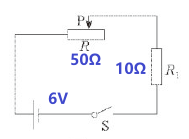
\includegraphics[width=0.3\textwidth]{img/0056.png} \\	
		串联电路中: \\
		- 电阻R1两端的电压 U1 =I × R1 \\
		- 电阻R2两端的电压 U2 =I × R2 \\
		- 串联电路的电压 U =U1+U2 		
		- 电流处处相等 \\
		\begin{align*}
			& U=U_1+U_2=IR_1+IR_2=I\left( R_1+R_2 \right)\\
			& I=\frac{U}{R_1+R_2}=\frac{6V}{10\varOmega +50\varOmega}=0.1A\\
		\end{align*}	
	\end{tcolorbox}
	
	由上面的例题可以看出,\textbf{``串联电路"中, 通过某个电阻的电流, 或串联电路的``电流", 等于电源两端``电压"除以``各分电阻之和"}。 \\
	另外, \textbf{当``串联电路"中的一个``电阻"改变时, 电路中的``电流"及另一个电阻两端的``电压", 都会随之改变。}很多实际电路都利用了``串联电路"的这一特点。\\
	
	
	
	\begin{tcolorbox}[title = {例},boxrule={0.1em},colframe={black!10}, colback={black!3},colbacktitle={black!10},coltitle={black}]		
		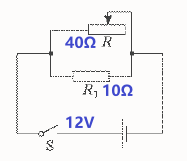
\includegraphics[width=0.3\textwidth]{img/0058.png} \\	
	并联电路中: 并联的支路电压相等
	\begin{align*}
			& I_1=\frac{U}{R_1}=\frac{12V}{10\varOmega}=1.2A\\
		& I_2=\frac{U}{R_2}=\frac{12V}{40\varOmega}=0.3A\\
		& \text{总电流}I=I_1+\text{I}_2=1.2A+0.3\text{A}=1.5\text{A}		
	\end{align*}	
	\end{tcolorbox}
	
	由上面的例题可以看出, \textbf{当``并联电路"中的一个支路的``电阻"改变时,这个支路的``电流"会变化、干路``电流"也会变化,但另一个支路的``电流"和``电压"都不变。} \\
	家庭电路中,各用电器采用``并联"形式连接到电源上,就是利用了``并联电路"的这一特点。\\
	
\vspace{1em} 


\subsection{电能 electric energy}

电能的单位, 叫``千瓦时"(即"度"), 符号是 kW·h.  \\
在物理学中,常用的能量单位是``焦耳"。\textbf{1千瓦时比1焦耳大得多。} 它们之间的关系是: 
\begin{align*}
	\boxed{
	1 kW·h = 1 \cdot 10^3 W \cdot 3600s = 3.6 \cdot 10^6 J	
	}
\end{align*}

用电器在一段时间内消耗的``电能",可以通过``电能表"(也叫``电度表")计量出来。\\

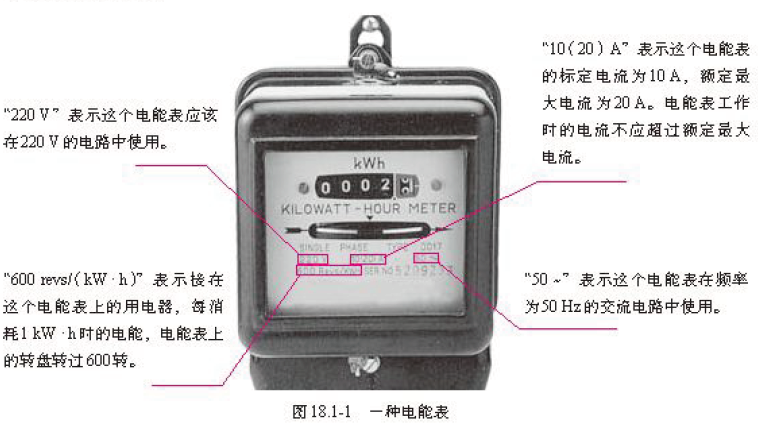
\includegraphics[width=1\textwidth]{img/0059.png} \\

电能表上显示的数字, 是表从开始记数, 到读数为止用去的电能。即, 为了计量一段时间内消耗的电能, 必须记录这段时间起始和结束时,  电能表上计数器的示数。前后两次示数之差,就是这段时间内用电的度数。 \\
例如,家中电能表, 在月初的示数是 3246.8 kW·h,月底的示数是 3265.4 kWh,这个月家里用电就是  $3265.4-3246.8= 18.6kW·h$ \\


目前, 常用的电能表是IC卡式的。用户将IC卡充值后插入电能表,电能表自动读取卡中的金额。一旦金额用完,电能表会切断电路. 所以表中的金额将要用完时,需要到银行为C卡储值,并重新将卡插人电能表。\\

\textbf{在实际生活中,为了计算电费方便, 读数时常常只读整数, 略去小数。}

\vspace{1em} 



\subsection{电功 : Work=U×I×time}

电能可以转化成多种其他形式的能量。\textbf{电能转化为其他形式的能的过程, 也可以说是电流``做功"的过程,有多少电能发生了转化, 就说电流做了多少功,即``电功"(electric work)是多少。}\\
例如: \\
- 电动机工作时,我们可以说``电能"转化成了``机械能",也可以说: 电流做功, 使电动机能够向外输出动能. \\
- 电炉工作时,可以说``电能"转化成了``内能",也可以说: 电流做功, 使电炉的内能增加. \\

在日常生活中,\textbf{我们常说消耗了多少电能,而很少说``电流做了多少功". 其实,两种说法是一样的。} \\

电流做功的多少, 跟电流的大小、电压的高低、通电时间的长短, 都有关系。\textbf{加在用电器上的电压越高、通过的电流越大、通电时间越长,电流做功越多。} \\
研究表明,当电路两端的电压为U,电路中的电流为I,通电时间为t时,\textbf{电功W(或者说消耗的电能)}为: 
\begin{align*}
	\boxed{
		\underset{\text{即消耗的电能}}{\underbrace{\text{电功}Work}}=\text{电压}U\cdot \text{电流}I\cdot \text{通电时间}t		
	}
\end{align*} \\




\begin{tcolorbox}[title = {例},boxrule={0.1em},colframe={black!10}, colback={black!3},colbacktitle={black!10},coltitle={black}]
例题有一只节能灯接在220 V的家庭电路中,通过它的电流为0.09 A, 计算这只灯使用5h, 会用电多少千瓦时?  \\
$W=UIt=220V \cdot 0.09A \cdot 5h = 0.099 \ kW·h$
\end{tcolorbox}


\vspace{1em} 

\subsection{$\text{电功率}Power=\frac{\text{电功}Work}{\text{完成这些电功所用的时间}time}=\frac{UIt}{t}=UI$}

\textbf{电功率 electric power: 表示电流做功的快慢. 电功率用P表示,它的单位是瓦特 watt ,简称瓦. 符号是W.} \\
不同的电器, 电功率各不相同。 比如有的电器是 24W的, 有的电器是 500W 的. \\

【电功率的单位】: \\
- 瓦: W \\
- 千瓦 kW: $1kW = 10^3 W$ \\
- 毫瓦 mW: $1W = 10^3 mW$ \\


【电功率的公式】: 
\begin{align*}
	\boxed{
	\text{电功率}Power=\frac{\text{电功}Work}{\text{完成这些电功所用的时间}time}=\frac{UIt}{t}=UI		
	}
\end{align*} \\
从公式可以看出: \textbf{电功率Power, 其实就是单位时间的电功Work值.} \\

我们变换一下公式, 就是: 
\begin{align*}
			\underset{\text{是}t\text{这段时间,\ 电流通过用电器所做的功.\ 即用电器消耗的电能}.}{\underbrace{\text{电功}Work<\text{焦耳}>}}=\underset{\text{电功率.即单位时间的电功值}}{\underbrace{Power<\text{瓦特}>}}\cdot \underset{\text{完成这些电功所用的时间}.}{\underbrace{time<\text{秒}>}}
\end{align*} \\

\textbf{如果把 Power 用千瓦为单位, time 用小时为单位, 那么它们相乘之后,就得到电能的另一个单位: 千瓦时(度)。 }
\begin{align*}
		\underset{\text{是}t\text{这段时间,\ 电流通过用电器所做的功.\ 即用电器消耗的电能}.}{\underbrace{\text{电功}Work<\text{千瓦时,即度}>}}=\underset{\text{电功率.即单位时间的电功值}}{\underbrace{Power<\text{千瓦}>}}\cdot \underset{\text{完成这些电功所用的时间}.}{\underbrace{time<\text{小时}>}}	
\end{align*}
\textbf{1千瓦时, 即电功率为1kW的用电器, 使用 1h 所消耗的电能。} \\



\begin{tcolorbox}[title = {例},boxrule={0.1em},colframe={black!10}, colback={black!3},colbacktitle={black!10},coltitle={black}]
一电视机的电功率是 150 W, 每天使用3h, 一个月用电多少千瓦时?(按30天计算) 
\begin{align*}
	& \text{电功}W=\text{电功率}P\cdot \text{用电时间}t \\
	& =150W\cdot 30\text{天} \\
	& =0.15\ kW\cdot 30\text{天}\cdot 3\text{小时}\\
	& =13.5<kW\cdot h>
\end{align*}
\end{tcolorbox}




【额定电压, 额定频率】:\\
不同用电器的``电功率" 一般不相同。那么,同一个用电器工作在不同的电压下, 它的电功率总是一样的吗? \\

实验: 取一个标有 36V, 25W 的灯泡。把它接在 36V 的电路中,它正常发光; 把它接在 24V 的电路中,它发光暗淡; 把它接 在40V 的电路中,它发光强烈. \\

实验表明, \textbf{在不同的电压下, 同一个用电器的电功率不一样大 : 用电器实际的电功率, 随着它两端的电压而改变。} \\
\textbf{既然如此,我们就不能泛泛地说一个用电器的``电功率"是多大,而要指明电压。}\\

→ 用电器正常工作时的电压, 叫做``额定电压" rated voltage. \\
→ 用电器在``额定电压"下工作时的``电功率", 叫做``额定功率" rated power. \\

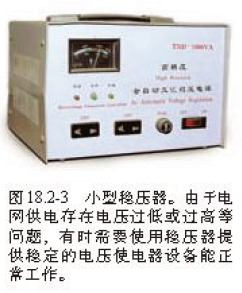
\includegraphics[width=0.3\textwidth]{img/0060.png} \\

- 节能灯上标着 220V, 24w,表示``额定电压"是220 V,``额定功率"是24 W. \\
- 电熨斗上标着 220V, 500w,表示``额定电压"是220 v,``额定功率"是500 W. \\

\textbf{我们使用各种用电器时, 一定要注意它的``额定电压",只有在``额定电压"下用电器, 才能正常工作}: \\
→ 实际电压偏低,用电器的``电功率"低,就不能正常工作。 \\
→ 反之, 实际电压偏高,有可能损坏用电器。 \\


\vspace{1em} 


\subsection{焦耳定律: 热量$Q = I^2 R t $}

生活中,许多用电器接通电源后, 都伴有热现象产生。电流通过导体时, ``电能"转化成``内能", 这种现象叫做电流的``热效应"。 \\
电炉丝通过导线接到电路里,电炉丝和导线通过的电流相同。那么为什么电炉丝热得发红,而导线却几乎不发热? 换句话说, \textbf{电流通过导体时, 产生热的多少, 跟什么因素有关?} \\

实验表明: \\
→ \textbf{在电流相同、通电时间相同的情况下,``电阻"越大,这个电阻产生的热量越多。} \\
→ \textbf{在电阻相同、通电时间相同的情况下,通过一个电阻的``电流"越大,这个电阻产生的热量越多。} \\

电流产生的``热量", 跟``电流"、``电阻"和``通电时间"的关系, 就由``焦耳定律" Joule 1aw 来总结: \\
\textbf{电流通过导体产生的热量Q, 跟``电流I 的二次方"成正比, 跟``导体的电阻R"成正比, 跟``通电时间 t"成正比。这个规律叫做``焦耳定律".}
\begin{align*}
	\boxed{
		\underset{\text{电流产生的热量}}{\underbrace{Q}}=\underset{\text{电流}}{\underbrace{I}}^2\cdot \underset{\text{电阻}}{\underbrace{R}}\cdot t
			}
\end{align*} 

电流通过导体时, 如果``电能"全部转化为``内能", 而没有同时转化为其他形式的能量, 那么,电流产生的热量, 就等于消耗的电能W,即 Q =W =Ult. 再根据欧姆定律 U=IR,就得到: $\text{热量}Q=\text{电能}Work=\underset{=I\cdot R}{\underbrace{U}}\cdot I\cdot time=IRIt=I^2Rt$ \\

所以, 上面电炉的例子, 为什么通电后, 导线不热, 电炉丝热, 就是因为两者的电阻不同. 导线的电阻很小, lm长的电线, 电阻不过百分之几欧姆. 而电炉丝的电阻可达几十欧姆到上百欧姆。所以, 当通过的电流相等时,电炉丝很热, 而导线却不热。 \\



\begin{tcolorbox}[title = {例},boxrule={0.1em},colframe={black!10}, colback={black!3},colbacktitle={black!10},coltitle={black}]
一根$60 \omega$ 的电阻丝, 接在 36V 的电源两端,在5 min内, 会共产生多少热量? 
\begin{align*}
	\text{热量}Q=\underset{=\frac{U}{R}}{\underbrace{I}}^2\cdot Rt=\left( \frac{36V}{60\varOmega} \right) ^2\cdot 60\varOmega \cdot \left( 5\text{分钟}\cdot 60\text{秒} \right) =6480\ J	
\end{align*}
\end{tcolorbox}


\underline{}



\section{家庭电路}

我国家庭电路的电压是220 V. \\

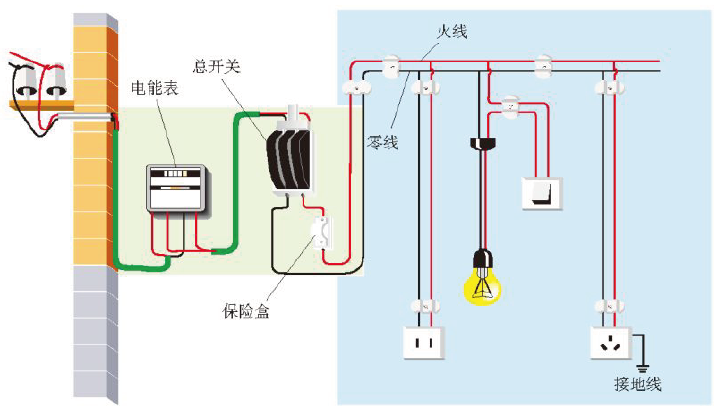
\includegraphics[width=1\textwidth]{img/0061.png} \\

上图是比较简单的家庭电路示意图,由两根进户线、电能表、总开关、保险装置、用电器、导线等组成。 \\
→ 输电线进户后, 首先接到``电能表"上,电能表用来显示所消耗的电能。 \\
→ 接下来是全户用电的总开关。当家庭电路需要修理时, 必须断开总开关,这时室内全部电路与外面的输电线分离,可以保证施工人员的安全。 \\
→ 总开关的后面是保险装置。熔丝(俗称``保险丝")是简易保险装置, 装在保险盒内。电流过大时熔丝会熔化, 切断电路, 对用电器起到保护作用。 \\
现在新建居民楼电路中的保险装置, 一般采用``空气开关",空气开关安装在电能表后, 如图19.1-1所示。\textbf{当电路中的电流过大时,空气开关自动断开, 切断电路,俗称``跳闸"。在找出电流过大的原因, 并把问题解决之后, 重新闭合``空气开关"就可以了。} \\

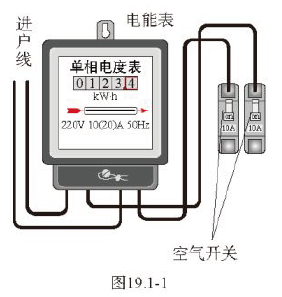
\includegraphics[width=0.3\textwidth]{img/0062.png} \\

→ 在电能表、总开关、保险装置之后,可以连接``用电器"。电路中还可以安装插座, 许多家用电器可以接在插座上。



【火线, 零线】: \\
\textbf{进户的两条输电线中,一条叫做``端线", 俗称``火线"; 另一条叫做``零线"。 零线在入户之前已经和大地相连。} \\
知道进户的两条线哪条是``火线"、哪条是``零线"非常重要。常用的方法是用``试电笔"来判断。 \\
一种试电笔的构造如图19.1-2所示。氖管中充有稀薄的氖气, 两端是两个金属电极。\textbf{当电极间的电压达到一定值时, 氖气会导电。当电流从一个电极流到另一个电极时, 氖气会发出红光。} \\

使用时, 手指按住笔卡,\textbf{用笔尖接融被测的导线(手指千万不能碰到笔尖)。} \\
→ 如果被测导线是``火线", 电流经过笔尖、电阻、氖管、弹簧, 再经过人体、经过大地, 流到零线,与电源构成闭合电路,氖管就会发光。 \\
→ 如果笔尖接触的是``零线",氖管中不会有电流,也就不会发光。 \\

\textbf{试电笔中, ``电阻"的作用十分重要。氖管发光只需很小的电流, 所以要在试电笔的电路中, 串联一个很大的电阻, 约有一百万欧姆。由于电流很小,使用试电笔时尽管电流通过人体,也不会对人造成伤害。} \\

另一种常见试电笔, 形状如螺丝刀(图19.1-3),使用时, 要用指尖抵住上端的金属帽。 \\

试电笔, 通常也用来检查电气设备的外壳是否带电。 \\

通常情况下,\textbf{家庭电路中各个用电器的通断, 不应该影响其他用电器的通断,所以用电器应该``并联"后接在电路中。控制用电器的开关, 要连接在``火线"和``用电器"之间。}



	
104
	
	
	
	
	
	
	
	
	
	
	
	
	
	
	
	
	
	
	
	
		

	


	
	
	
	
	
	
	
	
	
	
	
	
\end{document}